\section{Cải tiến về Hardware}
    Trong thiết kế phần cứng, phiên bản 1.0.0 mở rộng các chức năng, đặc biệt là mạng phân phối nguồn và quản lý nguồn, các cơ chế đọc tín hiệu, cải tiến layout và thiết kế cơ khí, vỏ hộp.

    \subsection{Những thay đổi về thiết kế PCB}
        \subsubsection{Thay đổi về Mức độ tích hợp linh kiện}\label{sec:thay_doi_muc_do_tich_hop_linh_kien}
            \begin{figure}[h]
                \centering
                \begin{subfigure}[b]{0.45\textwidth}
                    \centering
                    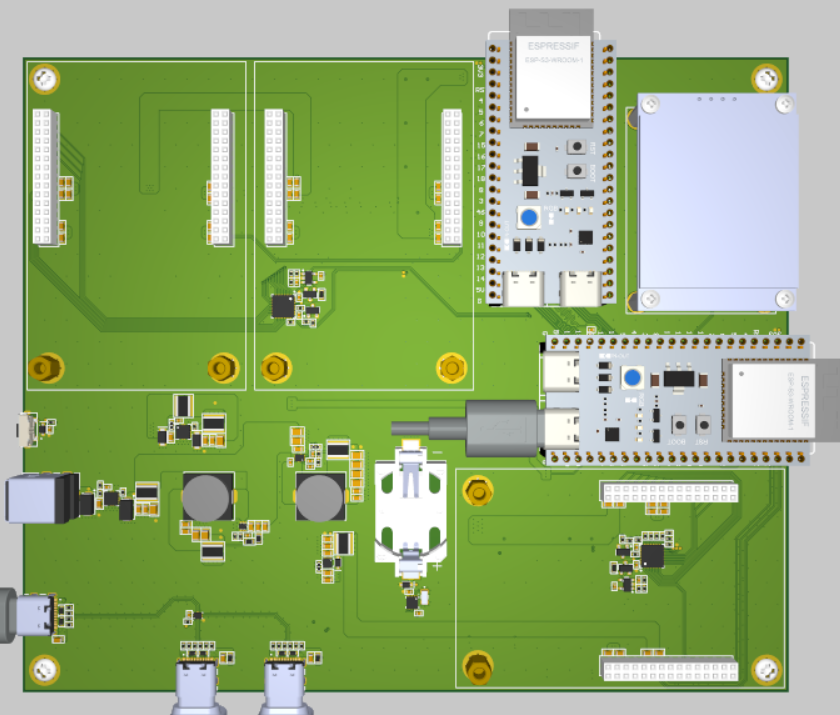
\includegraphics[width=\textwidth]{figures/iot_gateway_ver_prototype.png}
                    \caption{Phiên bản nguyên mẫu sử dụng module rời}
                \end{subfigure}
                % \hfill
                \hspace{1cm}
                \begin{subfigure}[b]{0.35\textwidth}
                    \centering
                    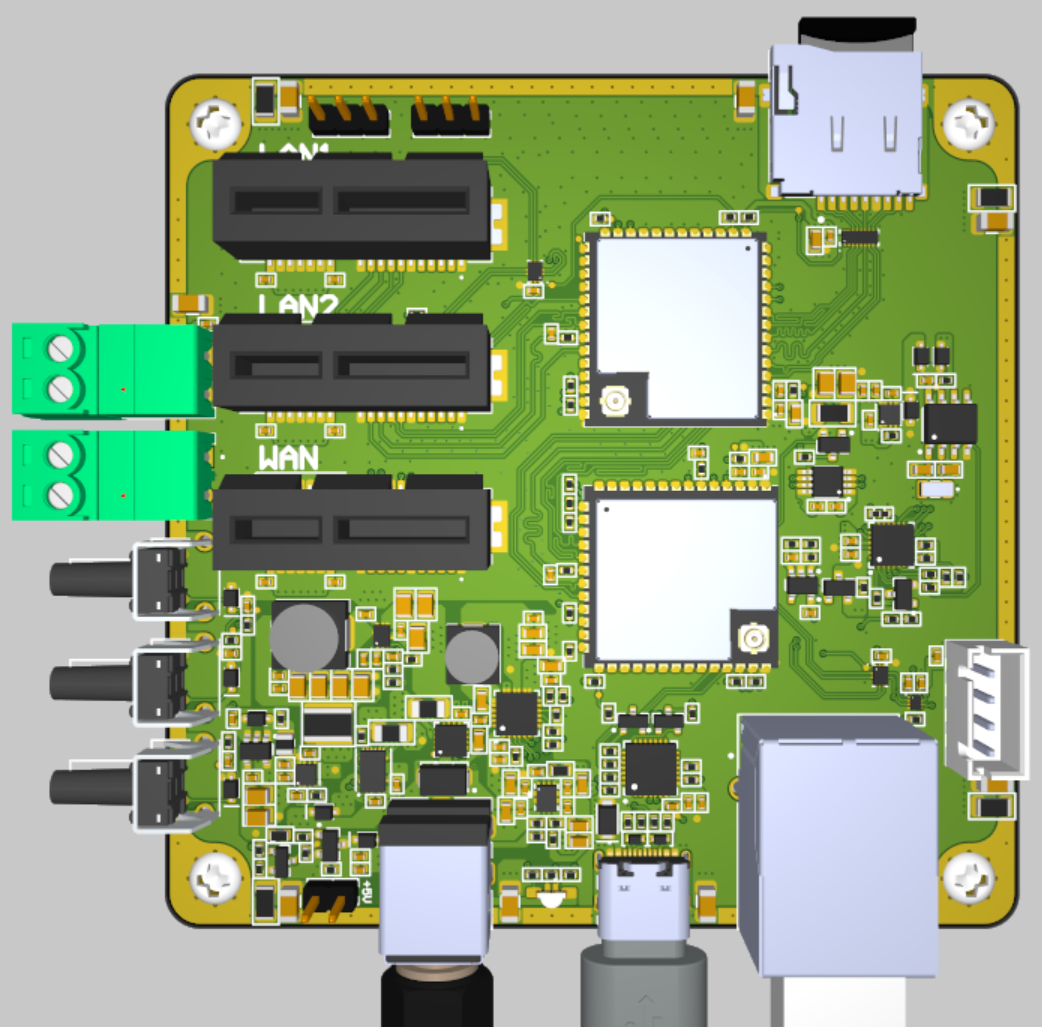
\includegraphics[width=\textwidth]{figures/iot_gateway_ver_1_0_0.png}
                    \caption{Phiên bản 1.0.0 tích hợp linh kiện}
                \end{subfigure}
                \caption{So sánh thiết kế giữa phiên bản nguyên mẫu và phiên bản 1.0.0}
            \end{figure}
            Trong phiên bản nguyên mẫu, nhằm giảm chi phí và thời gian phát triển, một số linh kiện được sử dụng ở dạng module rời. Tuy nhiên, trong phiên bản 1.0.0, đã có sự chuyển đổi sang việc tích hợp toàn bộ linh kiện trực tiếp trên PCB, giúp giảm kích thước tổng thể của gateway và cải thiện độ tin cậy của kết nối giữa các linh kiện.\par
            Có thể thấy rằng, ở phiên bản nguyên mẫu, các module rồi làm tăng đáng kể kích thước của board, làm hạn chế khả năng quy hoạch bố trí linh kiện, trong khi đó, ở phiên bản 1.0.0, việc tích hợp linh kiện đã giúp giảm đáng kể kích thước của board, tăng mật độ linh kiện, bố trí linh kiện tối ưu hơn, đồng thời cải thiện hiệu suất và độ tin cậy của hệ thống.

        \subsubsection{Thay đổi về Mạng phân phối nguồn}
            Mạng phân phối nguồn của phiên bản nguyên mẫu sử dụng nhiều mức nguồn khác nhau gồm 5.0V, 3.3V, 1.8V để cung cấp cho các thành phần của mạch, trong khi đó ở phiên bản 1.0.0, mạng nguồn chỉ sử dụng nguồn 3.3V làm nguồn chính, riêng nguồn 5.0V chỉ được sử dụng như nguồn phụ cho các ngoại vi khác như màn hình và quạt tản nhiệt.
            \begin{figure}[h]
                \centering
                \begin{subfigure}[b]{0.4\textwidth}
                    \centering
                    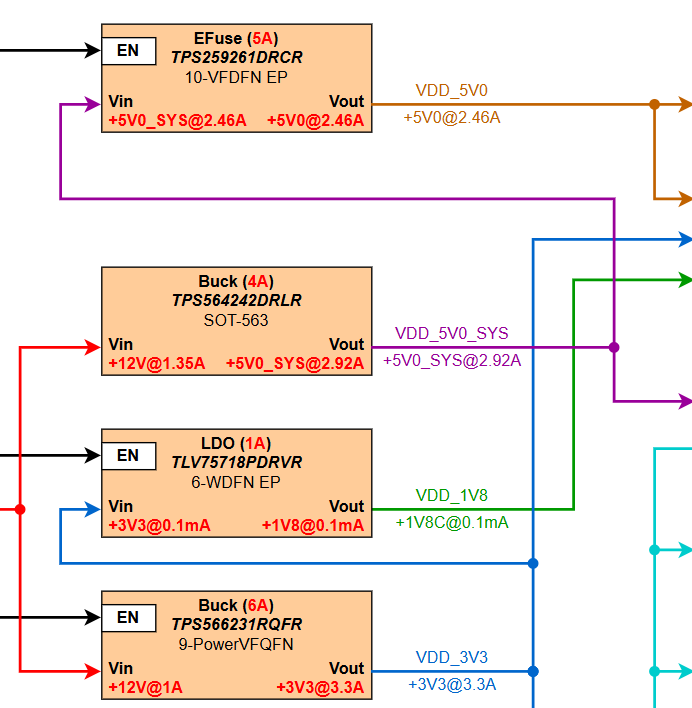
\includegraphics[width=\textwidth]{figures/power_network_ver_prototype.png}
                    \caption{Mạng phân phối nguồn của phiên bản nguyên mẫu}
                \end{subfigure}
                % \hfill
                \hspace{1cm}
                \begin{subfigure}[b]{0.4\textwidth}
                    \centering
                    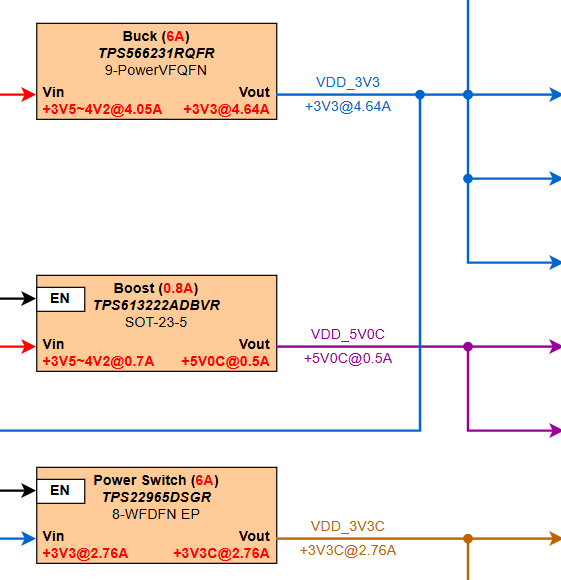
\includegraphics[width=\textwidth]{figures/power_network_ver_1_0_0.png}
                    \caption{Mạng phân phối nguồn của phiên bản 1.0.0}
                \end{subfigure}
                \caption{So sánh mạng phân phối nguồn giữa phiên bản nguyên mẫu và phiên bản 1.0.0}
            \end{figure}

            \begin{figure}[h]
                \begin{minipage}{0.3\textwidth}
                    \centering
                    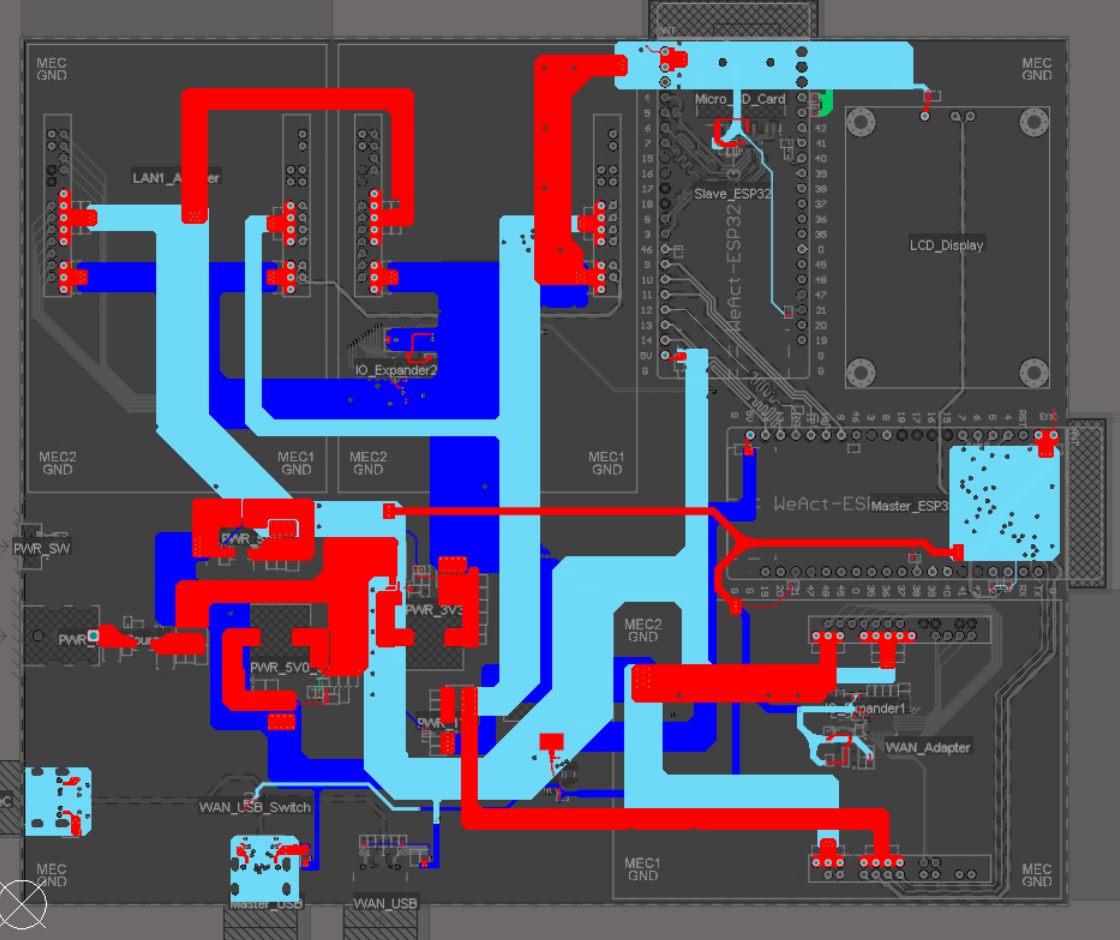
\includegraphics[width=\textwidth]{figures/power_network_layout_ver_prototype.png}
                    \caption{Layout của phiên bản nguyên mẫu}
                \end{minipage}
                \hfill
                \begin{minipage}{0.65\textwidth}
                Việc sử dụng một mạng nguồn nhiều mức trong phiên bản nguyên mẫu, cùng với sự hạn chế về khả năng quy hoạch bố trí linh kiện như đã được đề cập trong \autoref{sec:thay_doi_muc_do_tich_hop_linh_kien}, dẫn đến việc layout rất phức tạp. Có thể thấy rằng các đường nguồn được kết nối đan nhau chằng chịt trên nhiều layer.
                \end{minipage}
            \end{figure}
            \newpage
            \begin{figure}[h]
                \begin{minipage}{0.65\textwidth}
                Trong khi đó, ở phiên bản 1.0.0, việc sử dụng một mạng nguồn đơn giản hơn đã giúp giảm đáng kể sự phức tạp của layout. Đối với các module adapter sử dụng mức nguồn khác như 5.0V hoặc 1.8V thì sẽ được chuyển đổi từ nguồn 3.3V được tích hợp riêng trên mỗi module adapter, giúp giảm đáng kể sự phức tạp của mạng phân phối nguồn, tăng khả năng mở rộng các module adapter, đồng thời cải thiện hiệu suất và độ tin cậy của hệ thống.
                \end{minipage}
                \hfill
                \begin{minipage}{0.3\textwidth}
                    \centering
                    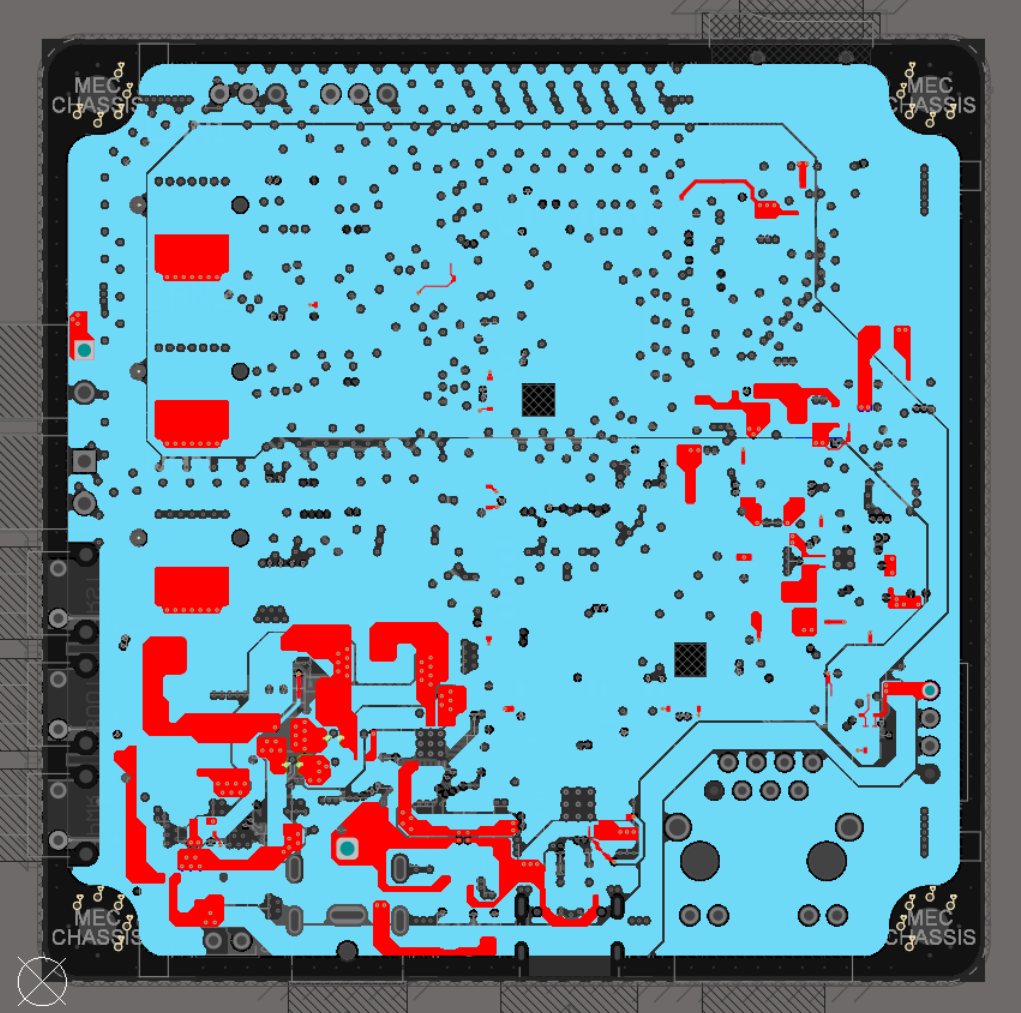
\includegraphics[width=\textwidth]{figures/power_network_layout_ver_1_0_0.png}
                    \caption{Layout của phiên bản 1.0.0}
                \end{minipage}
            \end{figure}

            \begin{figure}[h]
                \begin{minipage}{0.45\textwidth}
                    \centering
                    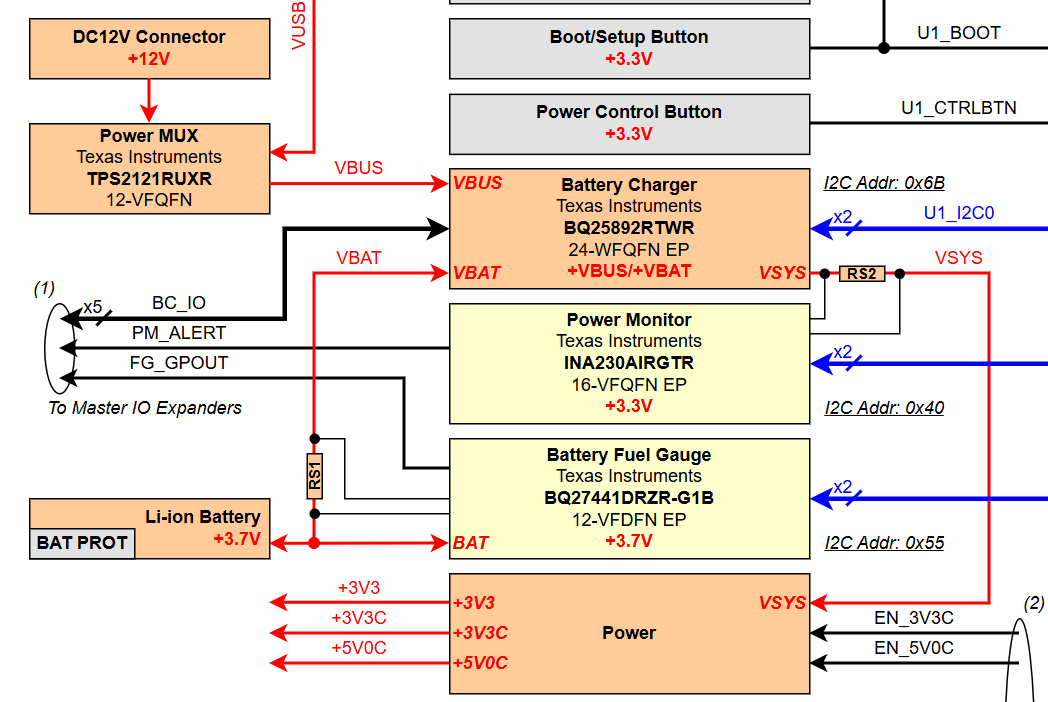
\includegraphics[width=\textwidth]{figures/power_management_ver_1_0_0.png}
                    \caption{Mạng quản lý nguồn của phiên bản 1.0.0}
                \end{minipage}
                \hfill
                \begin{minipage}{0.45\textwidth}
                    Từ mạng nguồn đơn giản hơn, thiết kế có thể tích hợp thêm các chức năng quản lý nguồn, bao gồm quản lý pin sạc, quản lý chất lượng nguồn, đo điện năng tiêu thụ, đáp ứng những yêu cầu cần thiết đối với một IoT gateway công nghiệp.
                \end{minipage}
            \end{figure}


        \subsubsection{Thay đổi về Cơ chế định danh module adapter}
            Trong phiên bản nguyên mẫu, các module adapter được định danh thủ công trên phần mềm cấu hình, ở phiên bản 1.0.0, đã có sự cải tiến bằng cách tích hợp một cơ chế định danh tự động cho các module adapter thông qua địa chỉ phần cứng được cấu hình sẵn trên mỗi module adapter. Cơ chế này được đề cập trong Phần Thiết kế Mạch Module Adapter, \autoref{par:sche_wanlan_adapter}.
        
        % \subsubsection{Thay đổi về Layout PCB}\label{sec:layout_pcb}

    \subsection{Những thay đổi về thiết kế cơ khí}
        \subsubsection{Thay đổi về Cơ chế kết nối module adapter}
            Trong phiên bản nguyên mẫu, các module adapter được thiết kế ở dạng cắm header nằm ngang, khiến cho thao tác tháo lắp rất khó khăn, chiếm diện tích không gian lớn, đồng thời khả năng kết nối tín hiệu kém, do đó trong phiên bản 1.0.0, các module adapter được thiết kế dạng module PCIe, giúp cải thiện đáng kể khả năng kết nối tín hiệu, đồng thời giảm diện tích không gian chiếm dụng, tăng tính tiện lợi trong thao tác tháo lắp.
            \newpage
            \begin{figure}
                \centering
                \begin{subfigure}{0.45\textwidth}
                    \centering
                    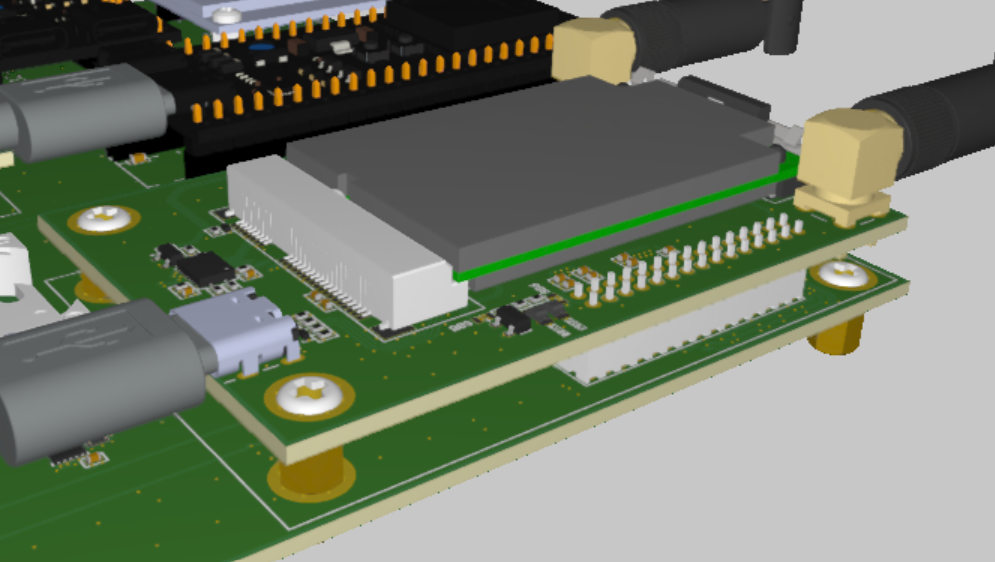
\includegraphics[width=\textwidth]{figures/module_adapter_connection_ver_prototype.png}
                    \caption{Cơ chế kết nối module adapter của phiên bản nguyên mẫu}
                \end{subfigure}
                % \hspace{1cm}
                % \hfill
                \begin{subfigure}{0.45\textwidth}
                    \centering
                    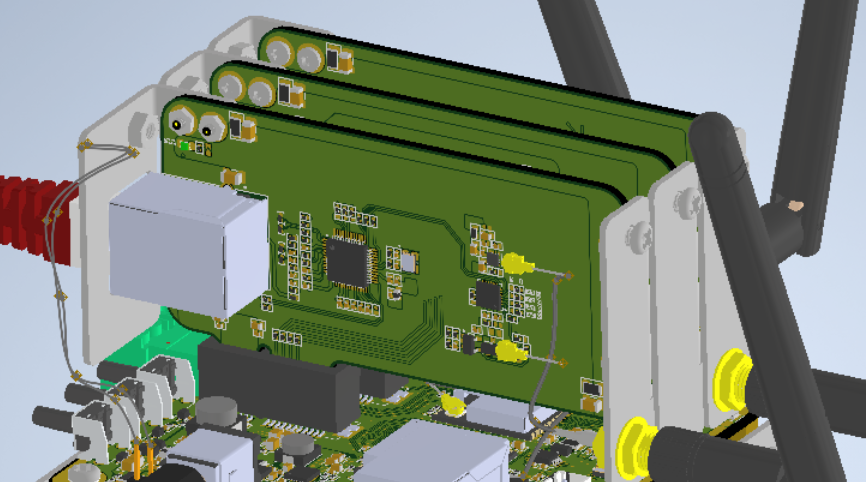
\includegraphics[width=\textwidth]{figures/module_adapter_connection_ver_1_0_0.png}
                    \caption{Cơ chế kết nối module adapter của phiên bản 1.0.0}
                \end{subfigure}
                \caption{So sánh cơ chế kết nối module adapter giữa phiên bản nguyên mẫu và phiên bản 1.0.0}
            \end{figure}

        \subsubsection{Thay đổi về Thiết kế vỏ hộp}
            
            \begin{figure}[h]
                \begin{minipage}{0.45\textwidth}
                    \centering
                    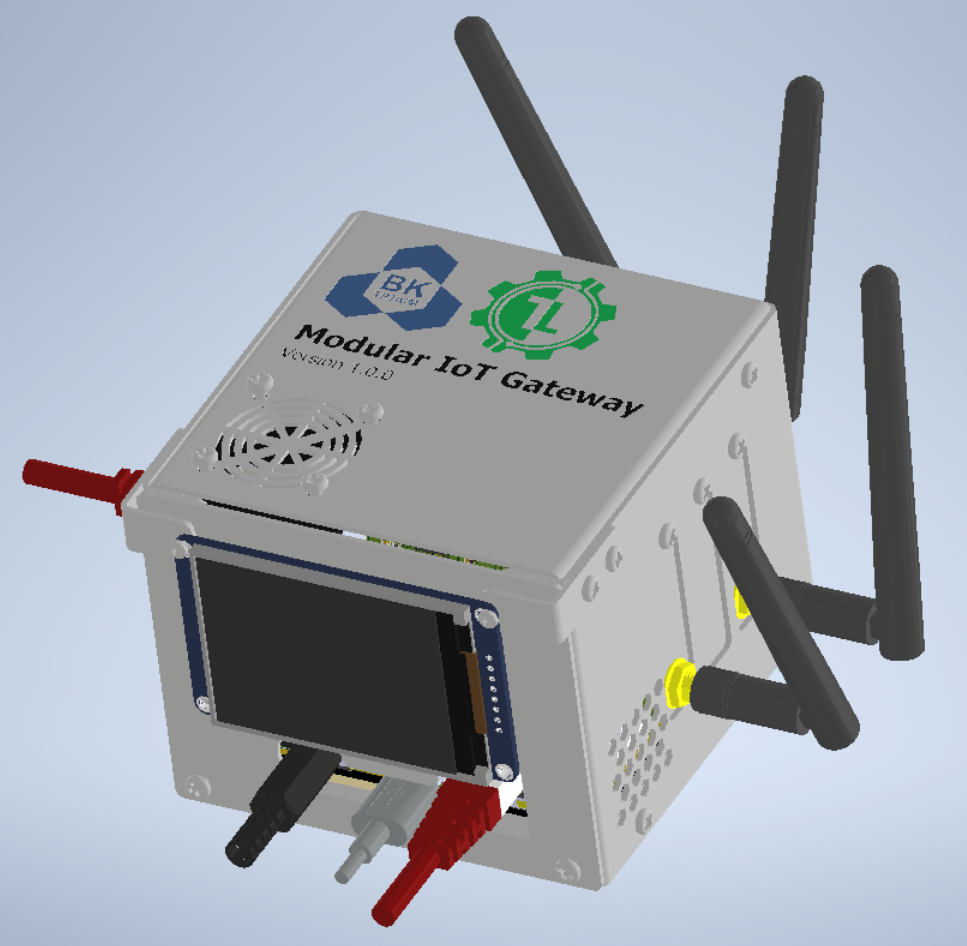
\includegraphics[width=\textwidth]{figures/modular_iot_gateway_with_case.png}
                    \caption{Thiết kế vỏ hộp của phiên bản 1.0.0}
                \end{minipage}
                \hfill
                \begin{minipage}{0.45\textwidth}
                    Một sản phẩm IoT Gateway công nghiệp yêu cầu về mức độ chống nhiễu, chống tĩnh điện, chống rò điện, do đó yêu cầu về một vỏ hộp chắc chắn, có khả năng chống chịu tốt là rất cần thiết. Vỏ hộp trong phiên bản này được thiết kế nhằm chống lại nhiễu điện từ và tĩnh điện, đồng thời hỗ trợ cơ chế kết nối các module adapter một cách dễ dàng và chắn chắn. Tuy nhiên, thiết kế vỏ hộp ở phiên bản hiện tại chưa được thiết kế để chống nước, chống bụi, do đó sẽ cần được cải tiến thêm trong các phiên bản tiếp theo để đáp ứng những yêu cầu khắt khe hơn đối với một IoT gateway công nghiệp.
                \end{minipage}
            \end{figure}